% Tik output from JumanG
\documentclass[class=minimal,border=0pt]{article}
\usepackage{tikz}
\pagestyle{empty}
\usepackage{verbatim}
\begin{document}
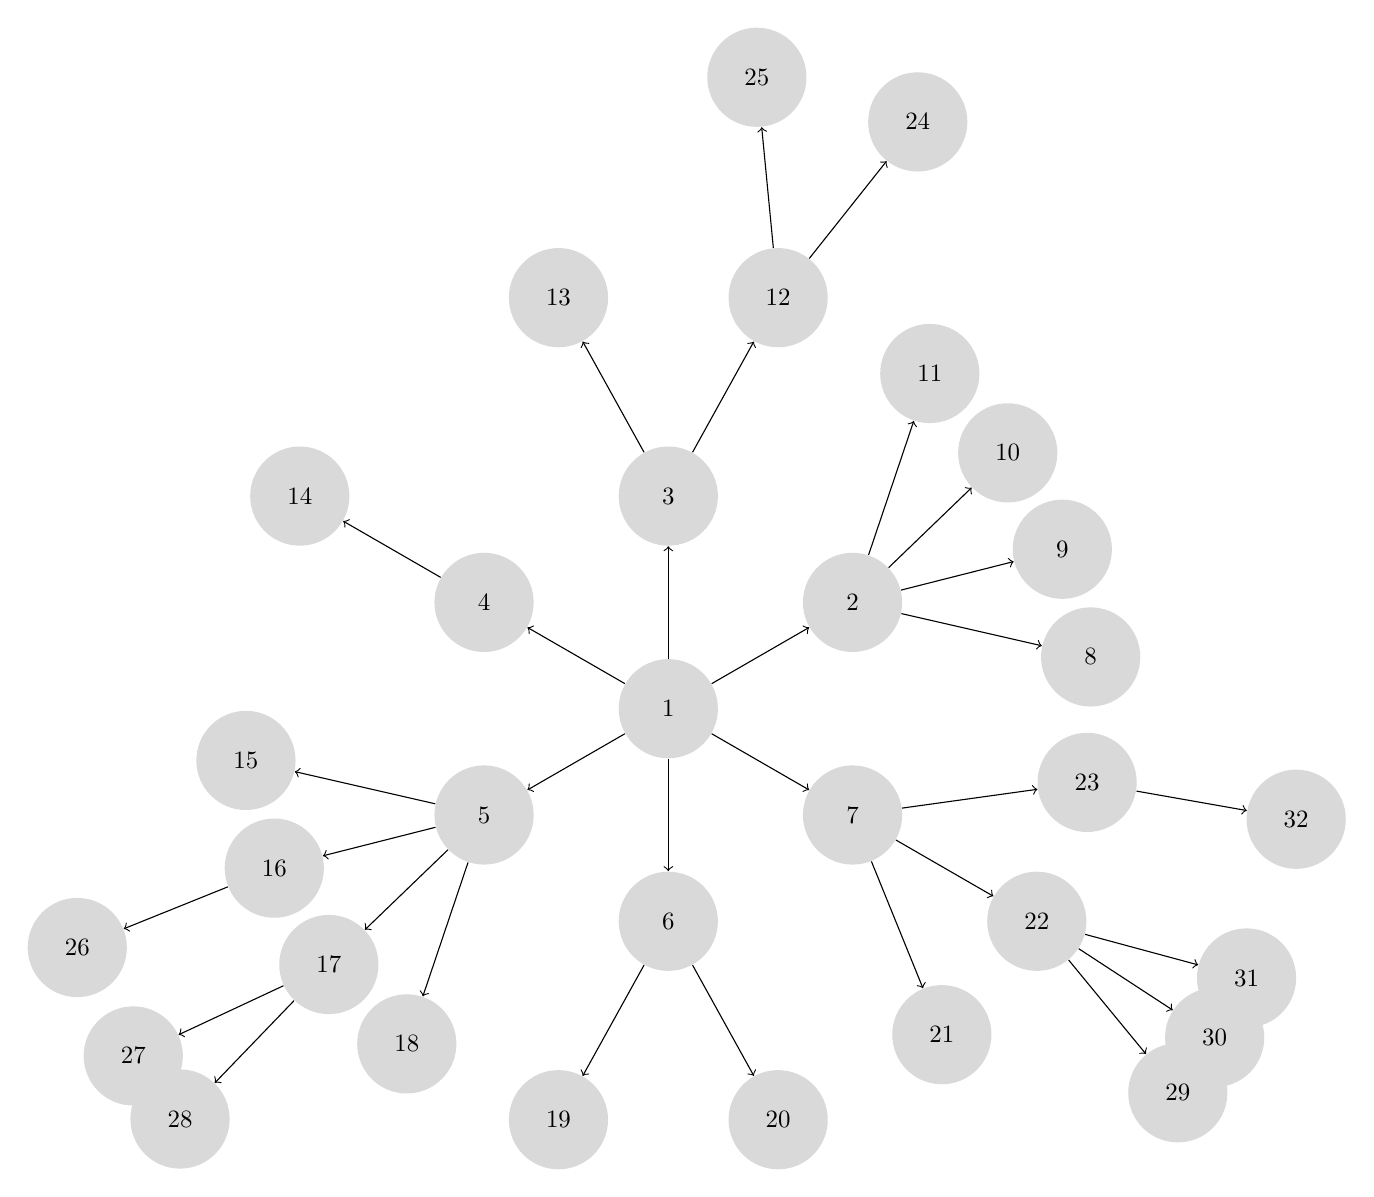
\begin{tikzpicture}[scale=0.90, transform shape]
	\tikzstyle{every node} = [circle, fill=gray!30, minimum size = 1.4cm]
	\node (24) at (3.52, 8.28) {24};
	\node (25) at (1.25, 8.91) {25};
	\node (26) at (-8.34, -3.37) {26};
	\node (27) at (-7.55, -4.90) {27};
	\node (20) at (1.55, -5.80) {20};
	\node (21) at (3.86, -4.60) {21};
	\node (22) at (5.20, -3.00) {22};
	\node (23) at (5.91, -1.04) {23};
	\node (28) at (-6.89, -5.79) {28};
	\node (29) at (7.19, -5.42) {29};
	\node (1) at (0.00, 0.00) {1};
	\node (3) at (0.00, 3.00) {3};
	\node (2) at (2.60, 1.50) {2};
	\node (5) at (-2.60, -1.50) {5};
	\node (4) at (-2.60, 1.50) {4};
	\node (7) at (2.60, -1.50) {7};
	\node (6) at (0.00, -3.00) {6};
	\node (9) at (5.56, 2.25) {9};
	\node (8) at (5.96, 0.73) {8};
	\node (11) at (3.69, 4.73) {11};
	\node (10) at (4.79, 3.61) {10};
	\node (13) at (-1.55, 5.80) {13};
	\node (12) at (1.55, 5.80) {12};
	\node (15) at (-5.96, -0.73) {15};
	\node (14) at (-5.20, 3.00) {14};
	\node (17) at (-4.79, -3.61) {17};
	\node (16) at (-5.56, -2.25) {16};
	\node (19) at (-1.55, -5.80) {19};
	\node (32) at (8.86, -1.56) {32};
	\node (31) at (8.16, -3.80) {31};
	\node (30) at (7.71, -4.64) {30};
	\node (18) at (-3.69, -4.73) {18};
	\draw [->] (22)--(29);
	\draw [->] (22)--(30);
	\draw [->] (22)--(31);
	\draw [->] (23)--(32);
	\draw [->] (1)--(2);
	\draw [->] (1)--(3);
	\draw [->] (1)--(4);
	\draw [->] (1)--(5);
	\draw [->] (1)--(6);
	\draw [->] (1)--(7);
	\draw [->] (3)--(12);
	\draw [->] (3)--(13);
	\draw [->] (2)--(8);
	\draw [->] (2)--(9);
	\draw [->] (2)--(10);
	\draw [->] (2)--(11);
	\draw [->] (5)--(15);
	\draw [->] (5)--(16);
	\draw [->] (5)--(17);
	\draw [->] (5)--(18);
	\draw [->] (4)--(14);
	\draw [->] (7)--(21);
	\draw [->] (7)--(22);
	\draw [->] (7)--(23);
	\draw [->] (6)--(19);
	\draw [->] (6)--(20);
	\draw [->] (12)--(24);
	\draw [->] (12)--(25);
	\draw [->] (17)--(27);
	\draw [->] (17)--(28);
	\draw [->] (16)--(26);
\end{tikzpicture}
\end{document}
